\chapter{Solar energy in South Africa and load curve covering concept}\label{Solar power in South Africa}
Almost all power that we use on our planet comes from the sun. Direct in form of radiation or indirect during wind, water and vegetation. Also the fossil power resources and reserves are stored energy from the sun in from of organic carbon compounds. 

The sun emits a power rate of about 3.83x10\textsuperscript{26}W. Of this total, only a tiny fraction, \SI{1367}{\watt\per\square\metre} (solar constant) reaches the Earth’s atmosphere. The solar radiation is reduced by absorption and reflection effects in the atmosphere.  The reduction is about \SI{30}{\percent} on a clear day and about \SI{90}{\percent} on a very cloudy day. \cite{Stine2001a}

When taking an eye on the world map in Figure~\ref{WorldDNI} it can be noticed that some parts of the world receive much higher direct parts of the sun’s irradiation than others. In particular four regions worldwide are worth mentioning. The Atacama Desert in South America, the Mojave Desert in North America, a huge part of Australia and parts of the southern Africa. Therefore SA is one of the country with the highest potential for generating solar electricity in the world.

\begin{figure}[h!] 
\centering
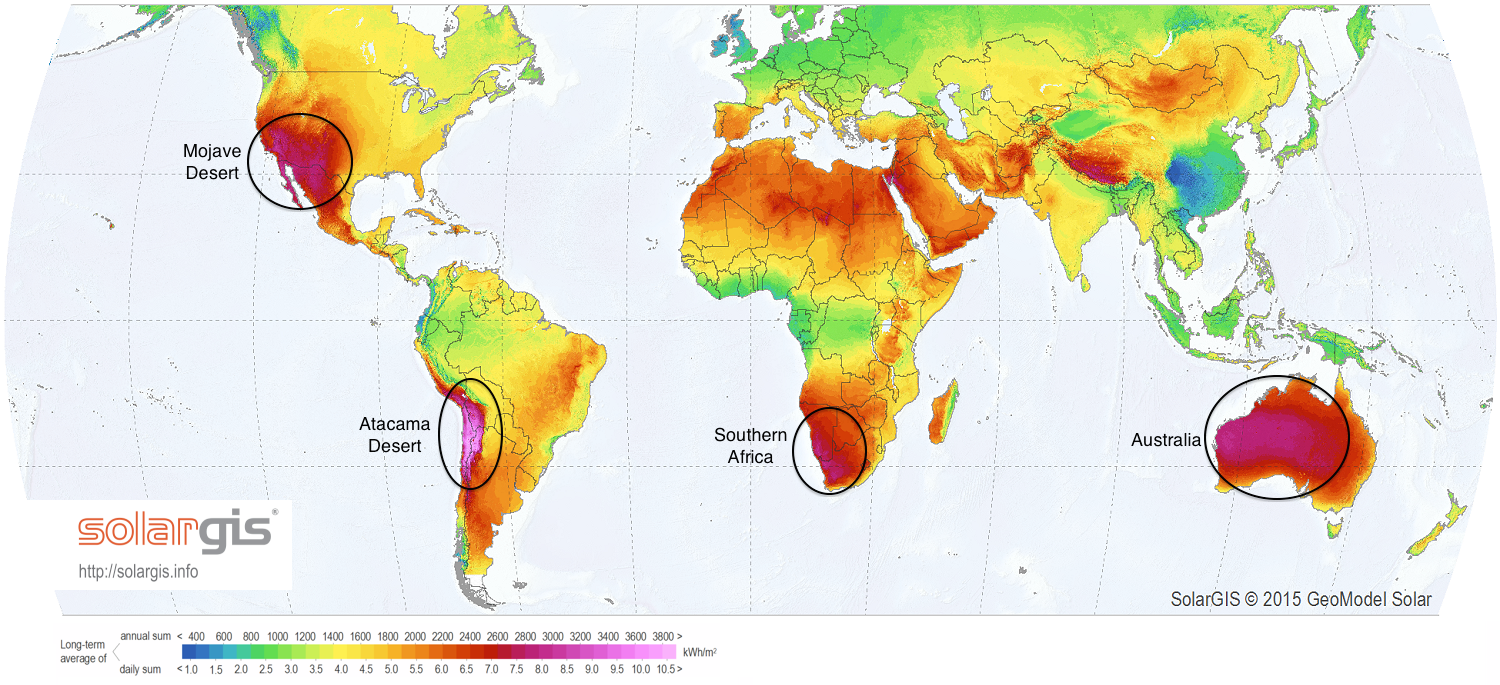
\includegraphics[width=1\linewidth]{FIG/WorldDNI}
\caption[World map of Direct normal irradiation.]{World map of Direct normal irradiation \cite{SolarGIS2015c}.}\label{WorldDNI}
\end{figure}  
\section{Solar irradiation in South Africa}
As shown above, solar irradiation is highly depending from the location. The solar irradiance of a specific location can be measured on-site by ground measurement devices or site-adapted by interpolated satellite data, which is validated with other ground measurement devices. Thereby is the direct and indirect as well as the total sun irradiance crucial. These solar irradiation parameter are here defined:
\begin{itemize}
\item \textbf{Global Horizontal Irradiance (GHI)} in \si{\watt\hour\per\square\metre\year} or \si{\watt\per\square\metre}: GHI is the total amount of shortwave radiation received from above by a horizontal surface. It includes direct (beam) and a diffuse (scattered) irradiation. This value is of particular interest to PV or solar water heater with a fixed inclined angle.
\item \textbf{Direct Normal Irradiance (DNI)} in \si{\watt\hour\per\square\metre\year} or \si{\watt\per\square\metre}: DNI is the amount of solar radiation received per unit area by a surface that is always held perpendicular (or normal) to the rays that come in a straight line from the direction of the sun at its current position in the sky. Diffuse irradiation is totally excluded from the DNI. This quantity is of particular interest to  installations that track the position of the sun.
\item \textbf{Diffuse Horizontal Irradiance (DHI)} in \si{\watt\hour\per\square\metre\year} or \si{\watt\per\square\metre}: DHI is the amount of radiation received per unit area by a surface that does not arrive on a direct path from the sun, but has been scattered by molecules and particles in the atmosphere and comes equally from all directions.
\end{itemize}
Furthermore is irradiance understood as instantaneous density of solar radiation incident on a given surface, typically expressed in \si{\watt\per\square\metre} and irradiation is the sum of irradiance over a time period expressed in \si{\joule\per\square\metre} or more commonly used in \si{\watt\hour\per\square\metre}. The connection between the solar radiation parameters is shown in Equation \ref{GL_GHI}. The angle $\theta_\text{z}$ is the angle between the direction of the sun and the zenith (directly overhead).
\begin{align}
GHI=DNI*\cos(\theta_{z})+DHI \label{GL_GHI}
\end{align}
The GHI is decisive for the power output of PV systems and the DNI for CSP systems. Figure\ref{irradiation} shows the solar GHI and the DNI data for SA. It is shown, that the ceiling value for GHI can be more than \SI{2300}{\kilo\watt\hour\per\square\metre\year}, whereas in some parts of the country the DNI  value attains about \SI{3200}{\kilo\watt\hour\per\square\metre\year}. This is significantly high than in the most regions worldwide, therefor SA is predestined for using solar technologies. The figure shows, that the southeastern coastline has predominantly the lowest irradiance values. The solar irradiation rise significant in the inland. The highest GHI can be find close to the Namibian boarder in the northeast of the country. The direct beam is also at highest in the western part of SA. The area around Springbok in the province Northern Cape has the highest DNI value of the country.

\begin{figure}[h!]
        \centering
        \begin{subfigure}[b]{0.5\textwidth}
                \centering
                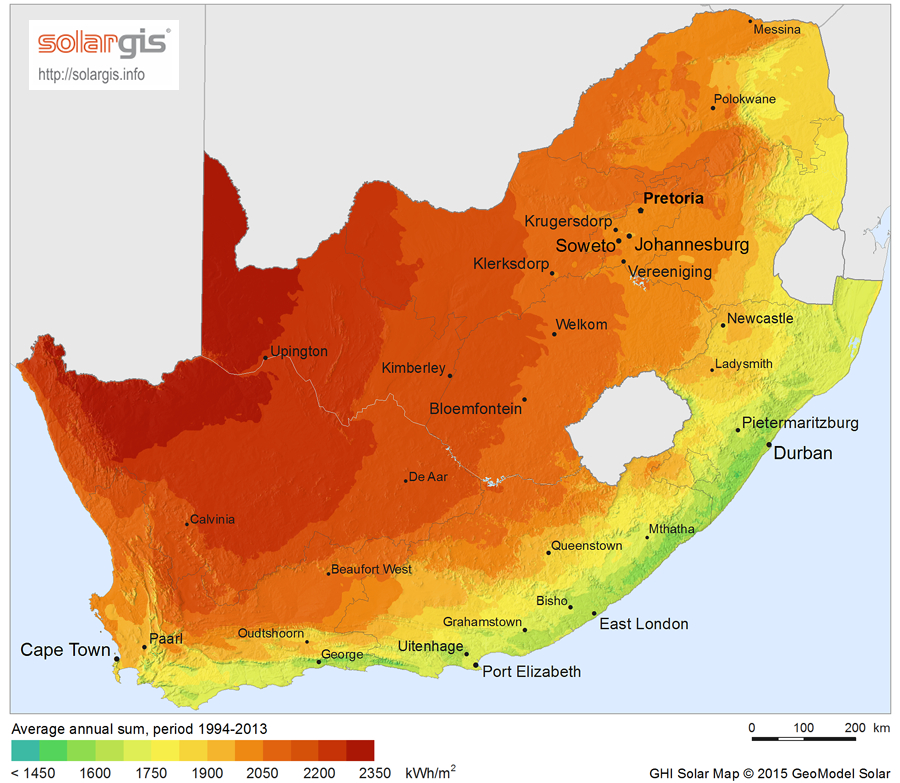
\includegraphics[width=1\textwidth]{FIG/SA_GHI}
                \caption{Global Horizontal Irradiation \cite{SolarGIS2015a}.}\label{fig:bild-links}
        \end{subfigure}%
        ~
        \begin{subfigure}[b]{0.5\textwidth}
                \centering
                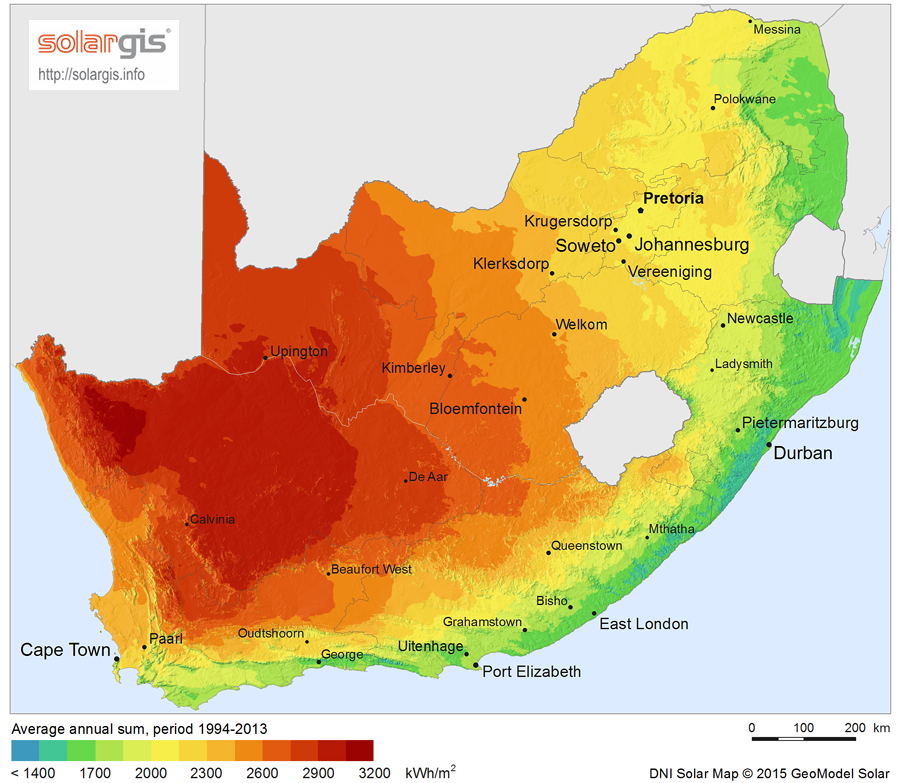
\includegraphics[width=1\textwidth]{FIG/SA_DNI}
                \caption{Direct Normal Irradiation \cite{SolarGIS2015b}.}\label{fig:bild-rechts}
        \end{subfigure}
        \caption{Solar radiation maps of South Africa.}\label{irradiation}
\end{figure}
Both maps demonstrates, that the highest values of solar irradiation can be found in the northwestern part of SA, which allocated in the Northern Cape Province. Currently all CSP plants and about two-thirds of the PV systems of SA are developed in the Northern Cape \cite{Forder2015}. Thereby the region around the city of Upington is highly attractive, owning to the high irradiation value in connection with a reliable water access due to the Orange River and the possibility of a close access to the Eskom grid. 

Therefore the location parameter and weather data of Upington was selected for the simulation and calculations in this thesis \cite{WhiteBoxTechnologies2015}. The hourly values of GHI and DNI over a full year for Upington are shown in Figure~\ref{Upington_GHI/DNI}. The highest irradiance value during the summer are \SI{1199}{\watt\hour\per\square\metre} for GHI and \SI{1154}{\watt\hour\per\square\metre} for DNI. At the northern solstice, the highest irradiance is \SI{625}{\watt\hour\per\square\metre} for GHI and \SI{820}{\watt\hour\per\square\metre} for DNI. 

So it is obviously that the irradiation values demonstrates significant seasonal variation of GHI with high values in summer and low irradiation in winter, whereas the DNI shows a more balanced variation throughout the year. This mainly leads from the irradiation angle which is changing constantly during the year. 

\begin{figure}[!htbp]
        \centering
                \begin{subfigure}[b]{1\textwidth}
                \centering
                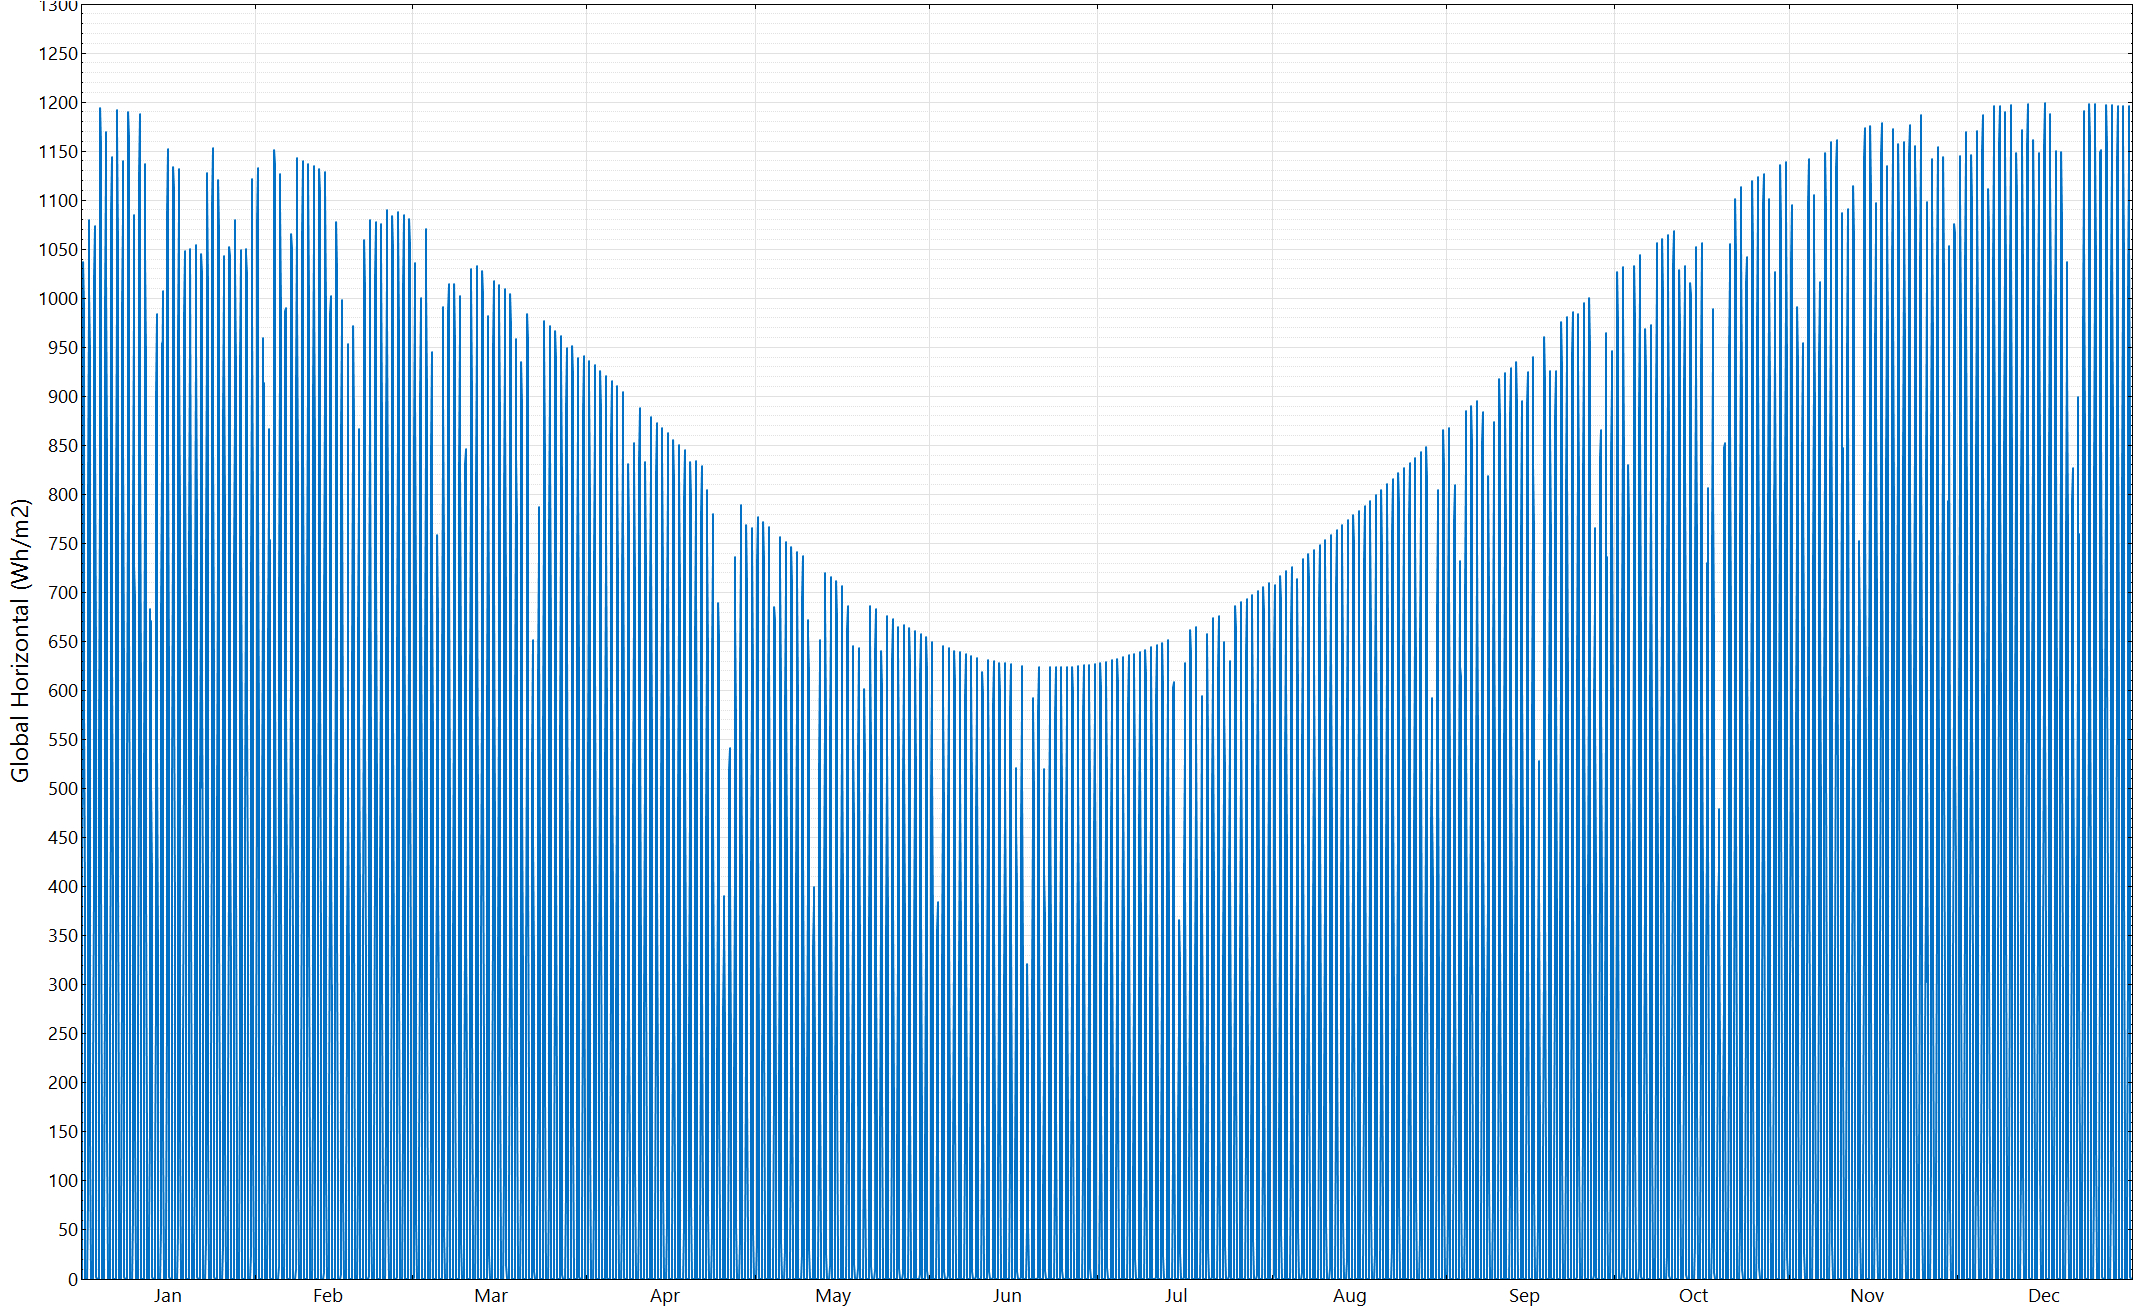
\includegraphics[width=1\textwidth]{FIG/Upington_GHI}
                \caption{Global horizontal irradiance}\label{Upington_GHI}
        \end{subfigure}%
\par\medskip % Linebreak      
        \begin{subfigure}[b]{1\textwidth}
                \centering
                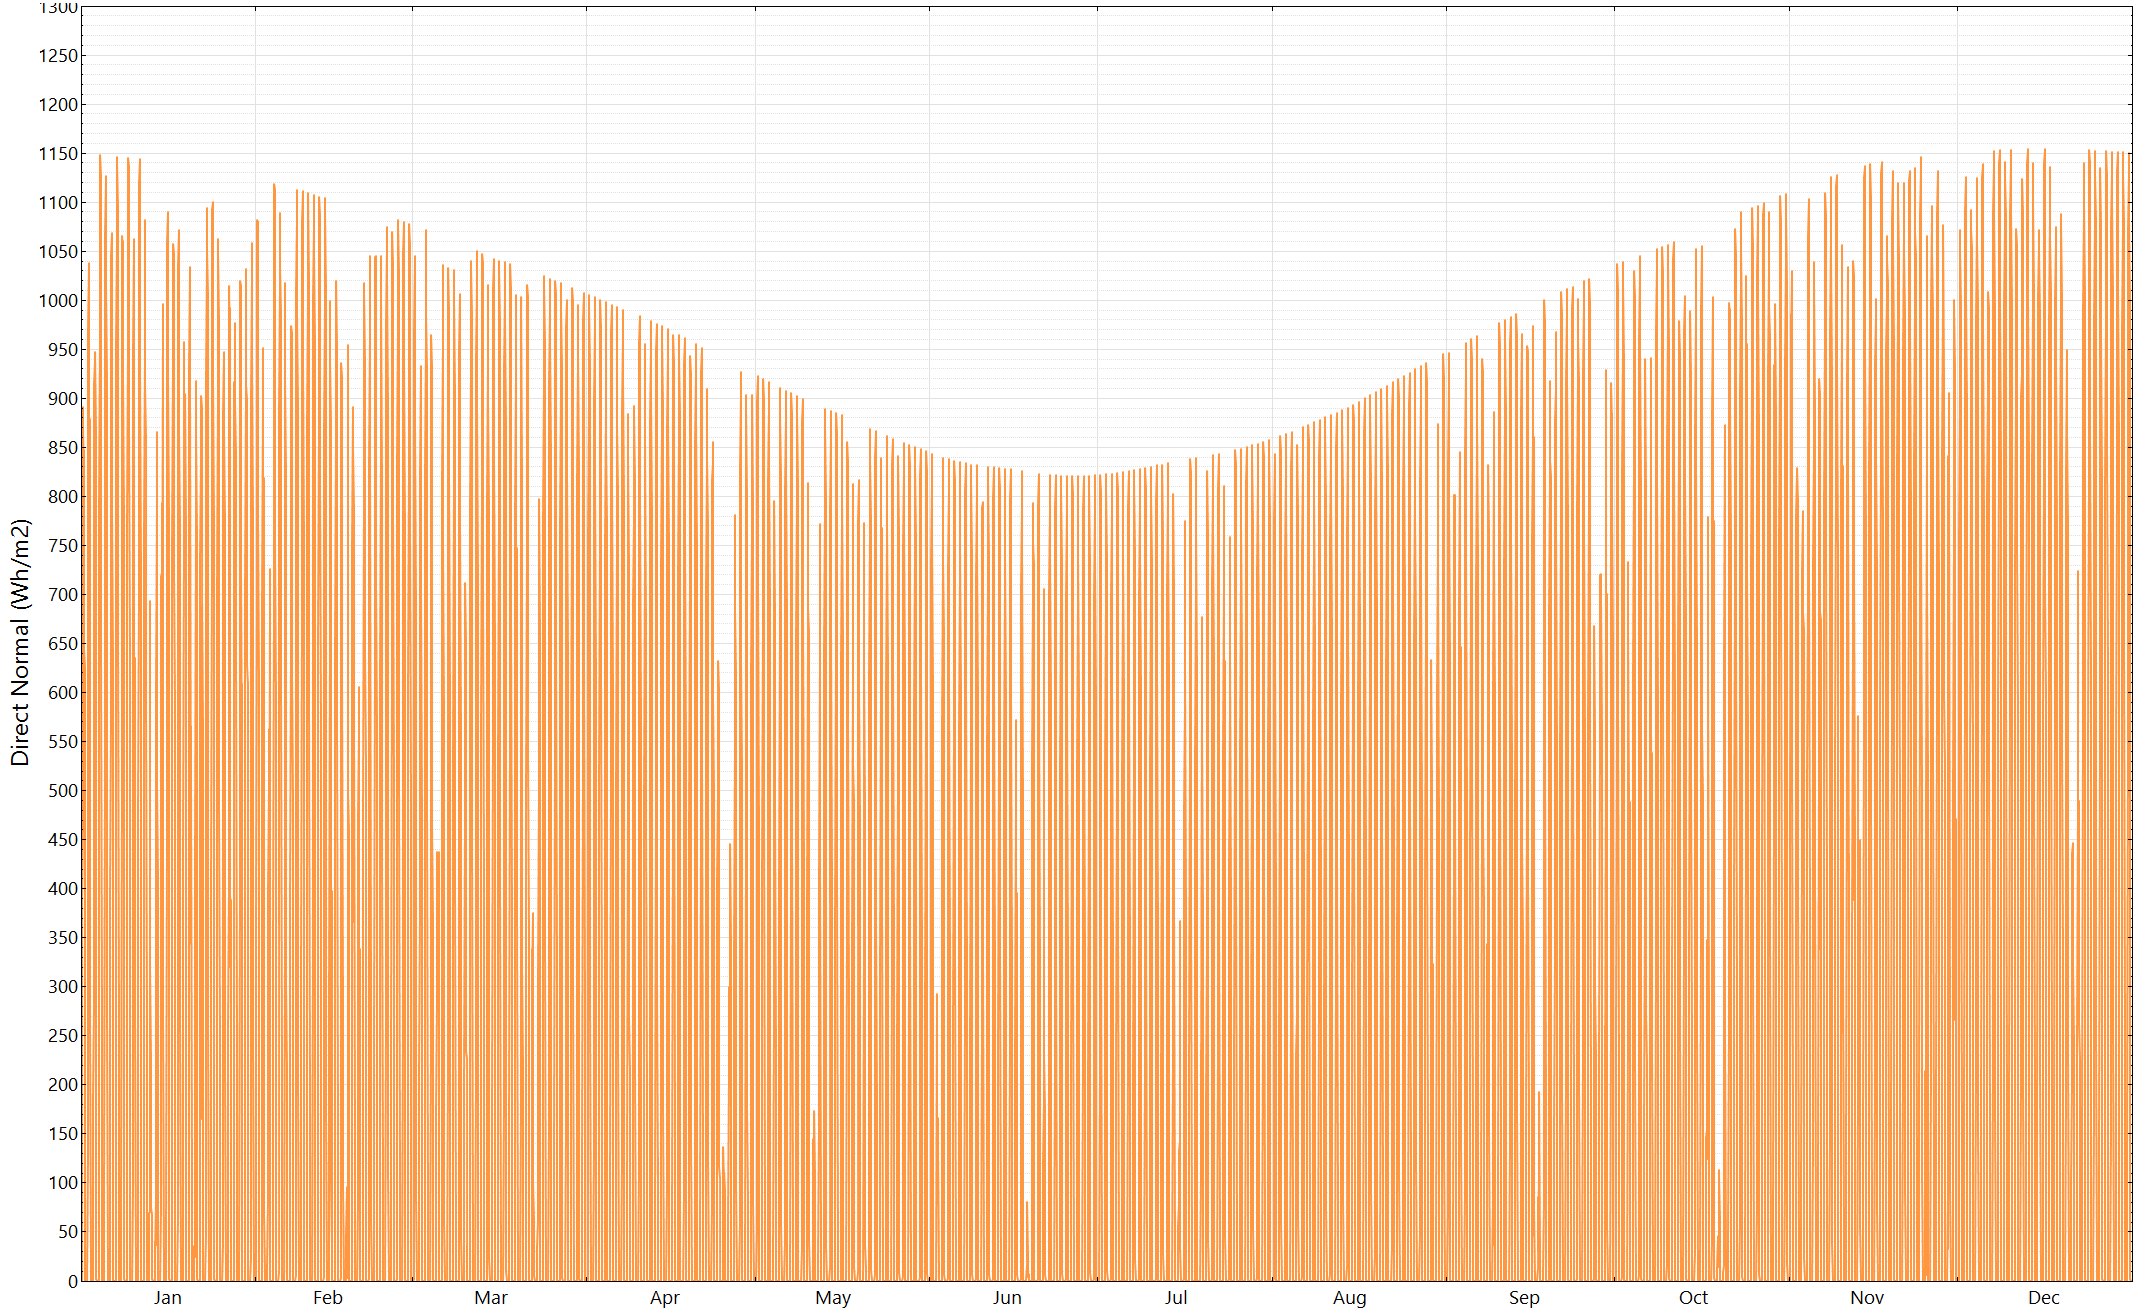
\includegraphics[width=1\textwidth]{FIG/Upington_DNI}
                \caption{Direct normal irradiance}\label{Upington_DNI}
        \end{subfigure}%

        \caption[Hourly values of irradiance over a full year from Upington used for the simulation.]{Hourly values of irradiance over a full year from Upington used for the simulation.}\label{Upington_GHI/DNI}
\end{figure}
The path of the sun during the year in Upington is characterize in Figure~\ref{SunPathUpington}. The solar path diagram depends on the geographical location by the position of longitude and latitude. The diagram apparent that the longest day in Upington has a duration of \SI{13}{h} and \SI{56}{minutes} with a maximum sun height of \SI{85.05}{\degree} while the shortest day has a duration of just \SI{10}{h} and \SI{19}{minutes} and a maximum sun height of \SI{35.93}{\degree}.

\begin{figure}[htbp]  
\centering
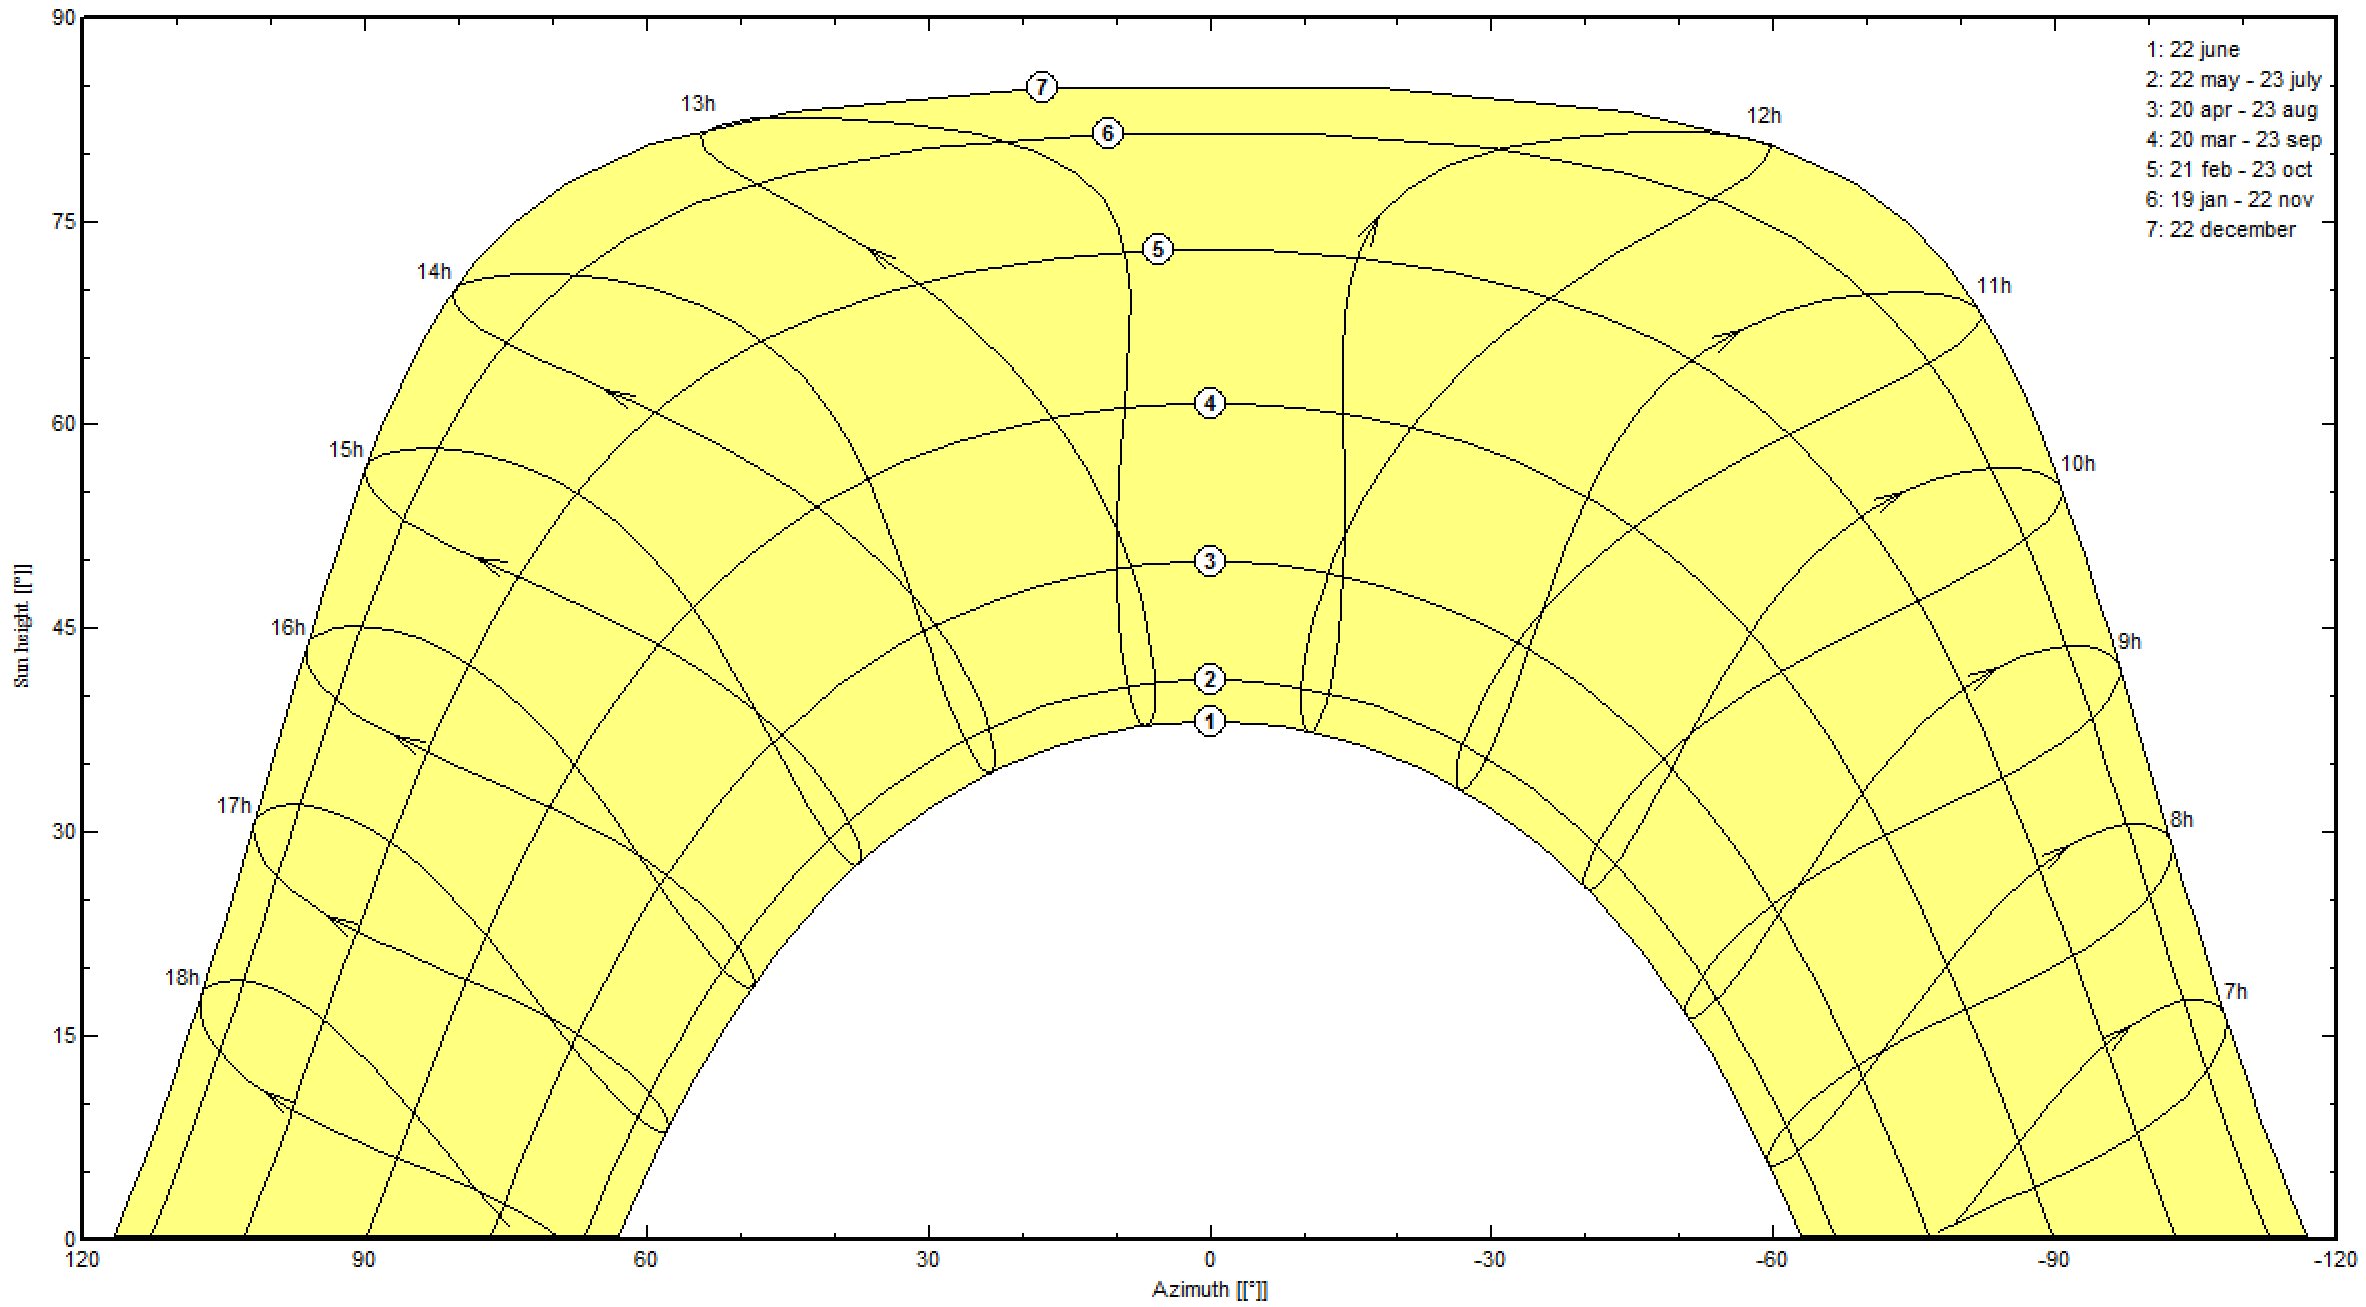
\includegraphics[width=1\linewidth]{FIG/SunPathUpington}
\caption[Solar path diagram for Upington.]{Solar path diagram Upington \cite{PVsystSA2015}.}\label{SunPathUpington}
\end{figure}
\pagebreak
From the hourly irradiation values concludes a annual sum of \SI{2280}{\kilo\watt\hour\per\square\metre\year} by GHI and an annuall DNI amount of \SI{2621}{\kilo\watt\hour\per\square\metre\year}. When comparing this for the simulation used data with the solar irradiation maps in Figure~\ref{irradiation} the annual sum of GHI is corresponding. But it must be noted that the annual sum of DNI from SolarGIS map \cite{SolarGIS2015b} is about \SI{200}{\kilo\watt\hour\per\square\metre\year} higher than the value which was used for the simulation in this thesis.

The weather data for the simulation are in EPW format (EnergyPlus Weather Data) and produced by White Box Technologies, Inc. \cite{WhiteBoxTechnologies2015}. The EPW files are data sets of hourly values of solar radiation and meteorological elements for a typical one-year period. These include air temperature (\si{\celsius}), dew point temperature (\si{\celsius}), relative humidity (\si{\percent}), atmospheric pressure(\si{\milli\bar}), global horizontal solar radiation (\si{\watt\per\square\metre}), diffuse horizontal solar radiation (\si{\watt\per\square\metre}), direct normal radiation (\si{\watt\per\square\metre}), wind speed (\si{\metre\per\second}), wind direction (\si{\degree}) and snow depth (\si{\metre}). The most relevant parameters for the simulation are summarized in Table \ref{tbl: Location}. 
 
\begin{table}[!h]  
  \centering
	\begin{tabular}{  p{4.0cm}  C{4.0cm}  C{3.0cm} } 
	\hline	
\textbf{Item}  & \textbf{Value} & \textbf{Unit} \\ \hline \hline
Location & Upington & -\\ 
Station ID &  684240& -  \\ 
Data source & White Box Technologies, Inc. (31.05.2015) & -\\ \hline
Latitude & -28.40 &$\,^{\circ}$N \\ 
Longitude &  21.27 &$\,^{\circ}$E \\ 
Elevation &  836 & m \\ 
Total GHI per year  &  2~280 & \si{\kilo\watt\hour\per\square\metre}\\ 
Total DNI per year &  2~621 & \si{\kilo\watt\hour\per\square\metre}\\ 
Total DHI per year &  516 & \si{\kilo\watt\hour\per\square\metre}\\ 
Mean temp. &  21 & \si{\celsius}\\ 
Mean wind speed & 3.3 & \si{\metre\per\second}\\ \hline
\end{tabular}
\caption[Location and characteristics for the simulation in SAM.]{Location and characteristics for the simulation in SAM.}\label{tbl: Location}
\end{table}
\pagebreak
\section{Current stage of solar power in South Africa}
South Africa started there expansion in the field of solar power plants with the first round of the REIPPPP in 2011. As it was mentioned before in Section~\ref{ElectricitySA} the REIPPPP has currently a capacity of \SI{5237}{\mega\watt} committed inclusive \SI{1899}{\mega\watt} PV systems and \SI{600}{\mega\watt} CSP plants. Additionally comes one CSP project with \SI{100}{\mega\watt} from Eskom which is not a part of the REIPPPP.

Figure \ref{Solar-map} shows the allocation of all currently committed solar power plants of the REIPPPP. Yellow marked are PV-power plants and CSP plants are marked in orange (some marks cover them mutually). The numbers in the single marks expose to which REIPPPP-Round it belongs.

Currently SA has 27 fully operational PV-power plants with a total capacity of \SI{1059.05}{\mega\watt} further six PV-power plants with in total of \SI{442.5}{\mega\watt} are under construction. \cite{Forder2015}

Most of the South African PV-power plants are allocated in the Northern Cape. So 29 out of 45 currently committed PV systems are located there. Five more each in the Western Cape and the North-West Province, three each in the provinces Free State and Limpopo, two in Eastern Cape and one more in the Eastern Cape. \cite{Forder2015}
\pagebreak

\begin{figure}[h!]
\centering
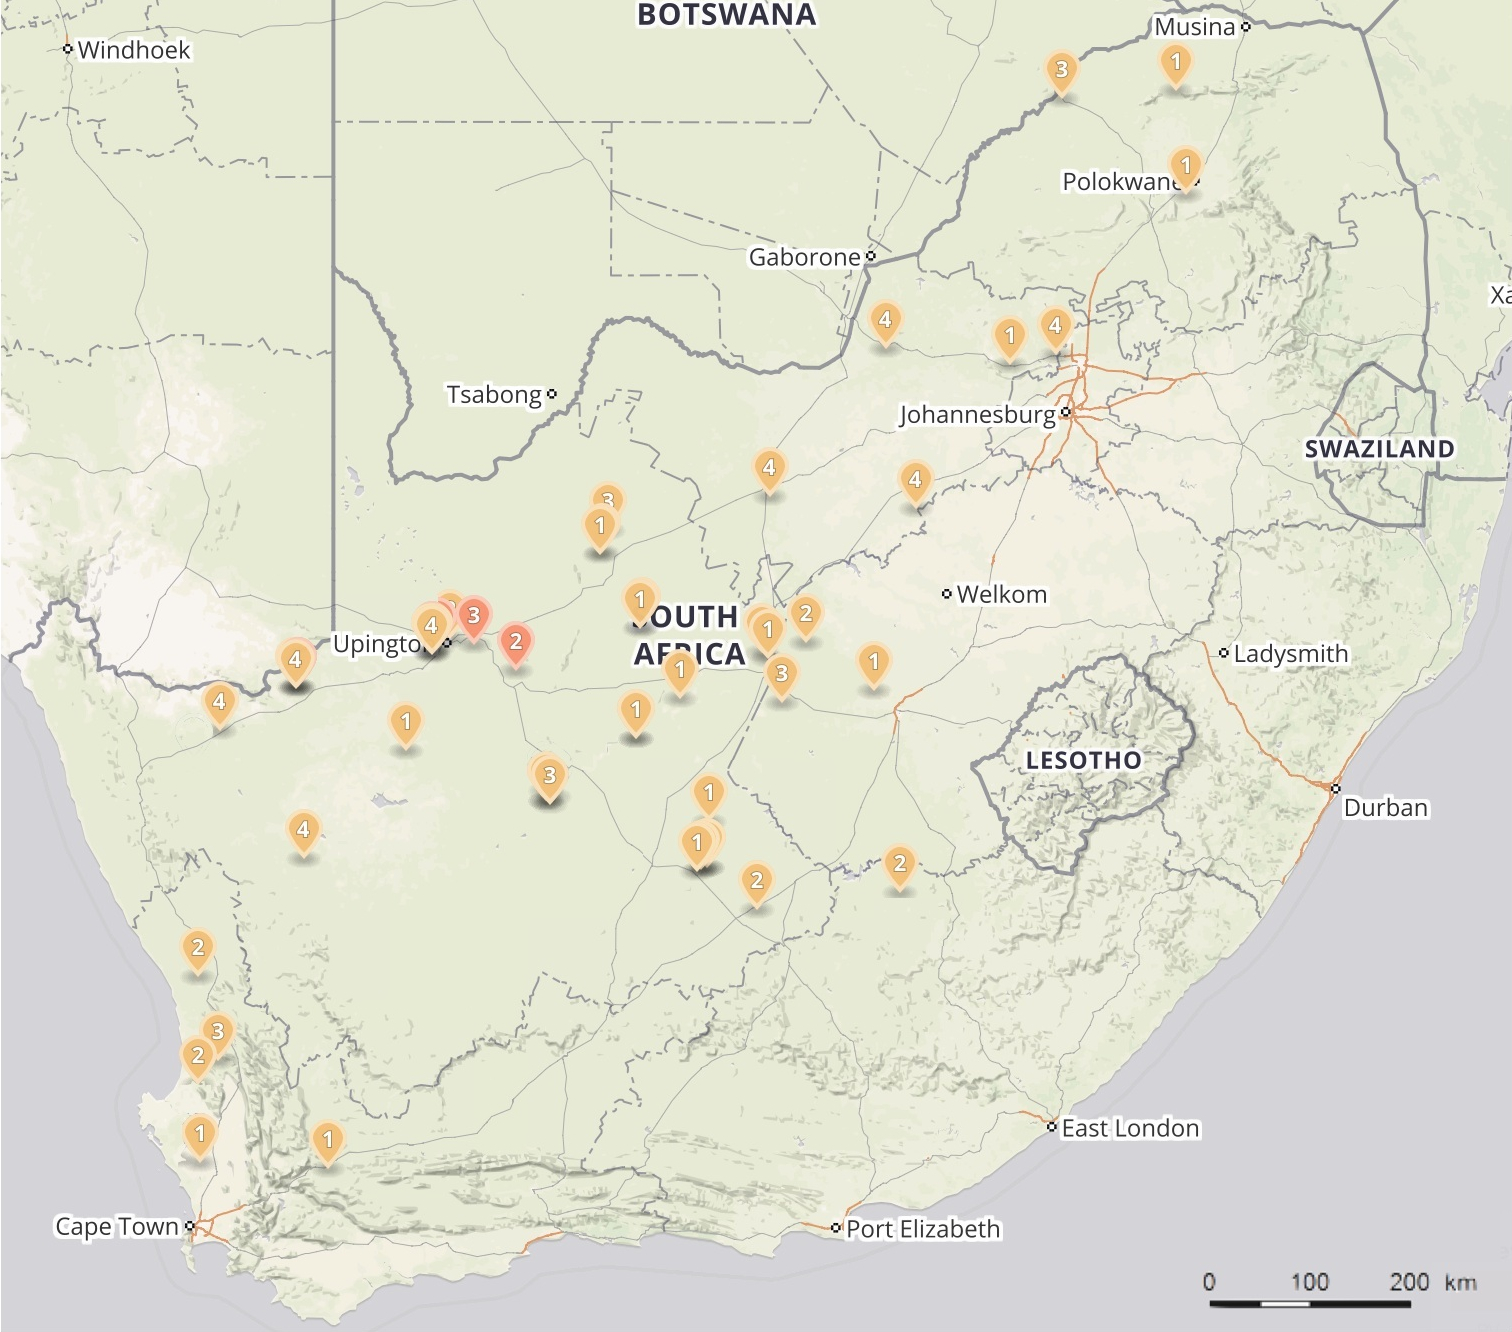
\includegraphics[width=1\linewidth]{FIG/Solar-map}
\caption[Allocation of all REIPPPP solar power plants in SA.]{Allocation of all REIPPPP solar power plants in SA \cite{Forder2015}.}\label{Solar-map}
\end{figure}

"KaXu Solar One" is the first and currently only full operational CSP plant in SA. It is using parabolic trough technology and a 2.5~h thermal energy storage for generating \SI{100}{\mega\watt} capacity. The CSP-plants "Khi Solar One" and "Bokpoort CSP Project" with a capacity of each 50~MW are under construction as well as the \SI{100}{\mega\watt} "Xina CSP South Africa" project. Further three CSP-plants are awaiting construction, they have all a capacity of each \SI{100}{\mega\watt}. As mentioned before, all eight CSP projects are located in the Northern Cape Province of SA. \cite{Forder2015}
\pagebreak
\section{System load in SA and prescribed solar power generation profil} \label{SystemloadinSA}
The South African supply structure is based on coal-fired thermal power plants, as it was shown in Section~\ref{ElectricitySA} before. But also the renewable energy supply is getting noteworthy for the supply structure in SA. When taking an eye on Figure~\ref{systemload} it can be noted that wind and PV power also makes a small share of the daily electricity supply. It has to be said that by the time of spring in 2014 the KaXu Solar One CSP plant was not completed and so CSP supply in SA doesn't exist. The reveals that the power demand in SA rises in the morning hours and is coming to a peak demand in the evening hours. The surplus energy during the night got compensated by pump storage and reduction by supply imports. 

\begin{figure}[htbp]  
\centering
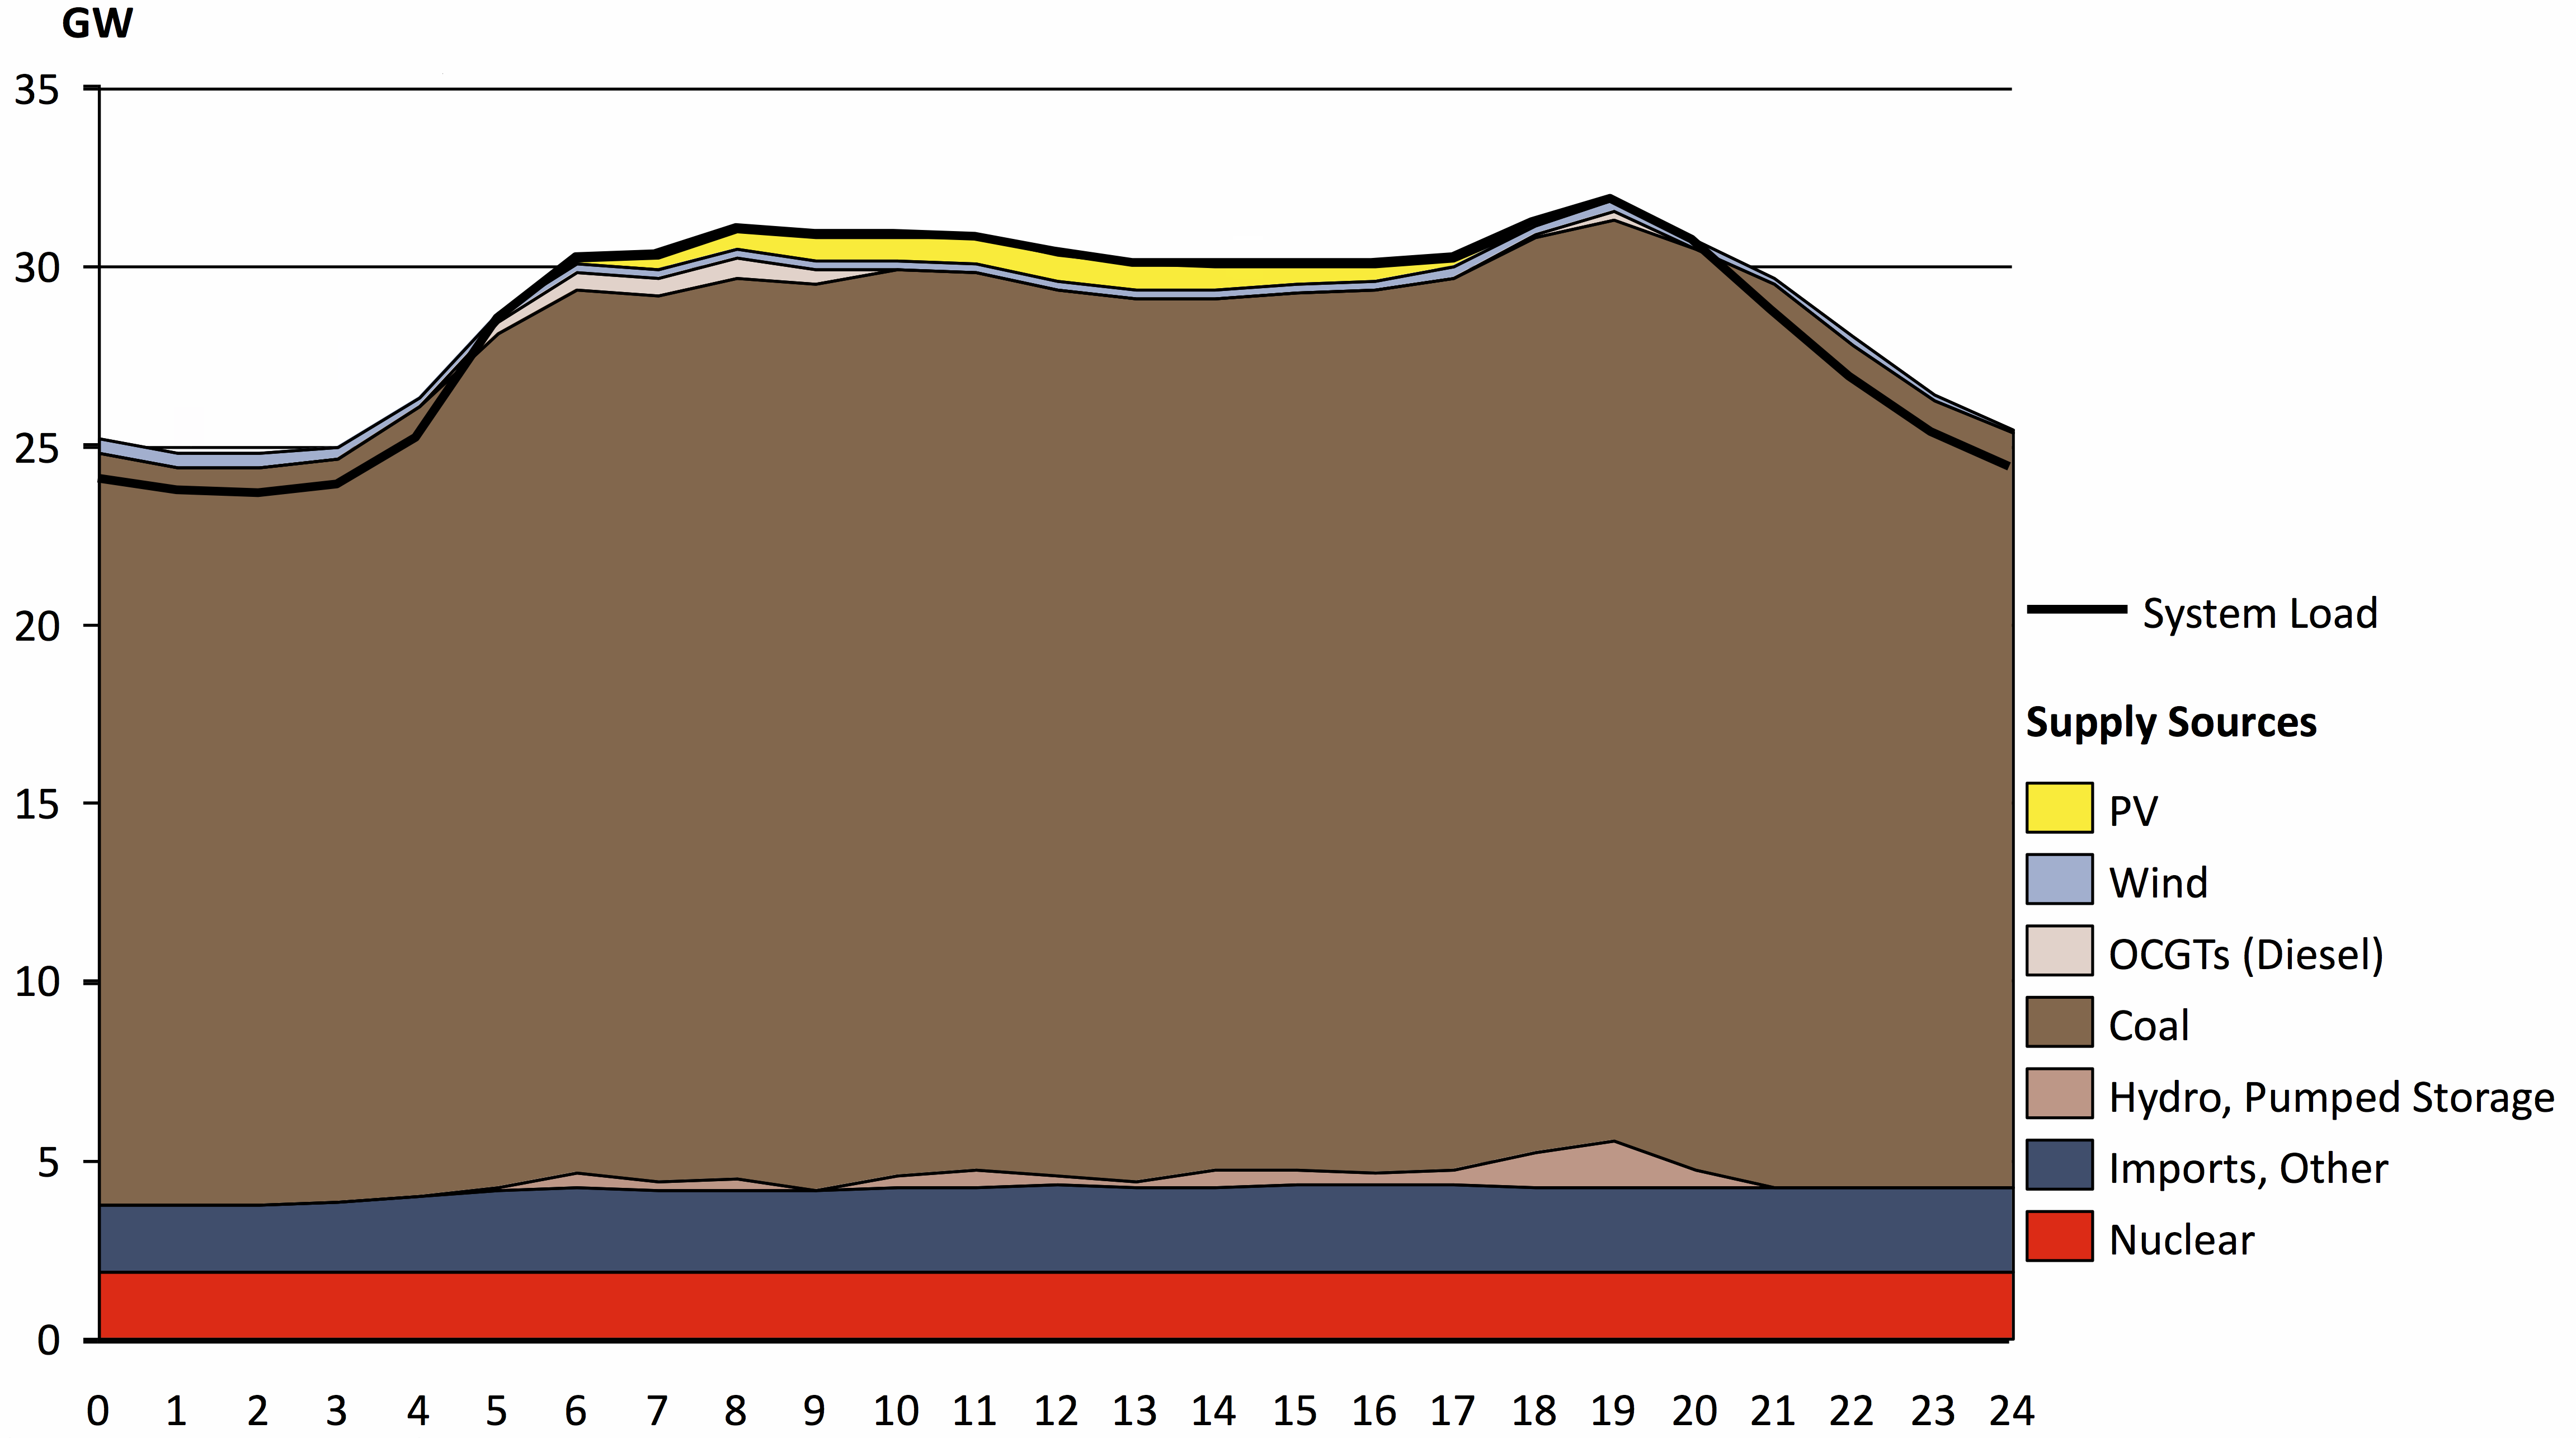
\includegraphics[width=1\linewidth]{FIG/systemload}
\caption[Actual South African supply structure for a spring day, the 17. October 2014.]{Actual South African supply structure for a spring day, the 17. October 2014 \cite{CSIR2015}.}\label{systemload}
\end{figure}
It is shown that the PV supply can support the South African demand during the day and reduces thereby the generation of coal-fired thermal power plants. But by the time of the daily peak demand, in the evening hours, the PV supply is coming to standstill, whereby this demand needs to be covered by pumped storage or expansive diesel driven open cycle gas turbines (OCGTs).

When taking an eye on the total unserved energy due to load shedding history of the first half year of 2015 in Figure~\ref{Load_shedding_sum} it is obviously that the capacity bottleneck in SA is mostly during the daytime and particularly during the evening peak hours till 22:00. This makes clear in which time period the support of new power plants is necessary for a secure electricity supply in SA.

\begin{figure}[htbp]  
\centering
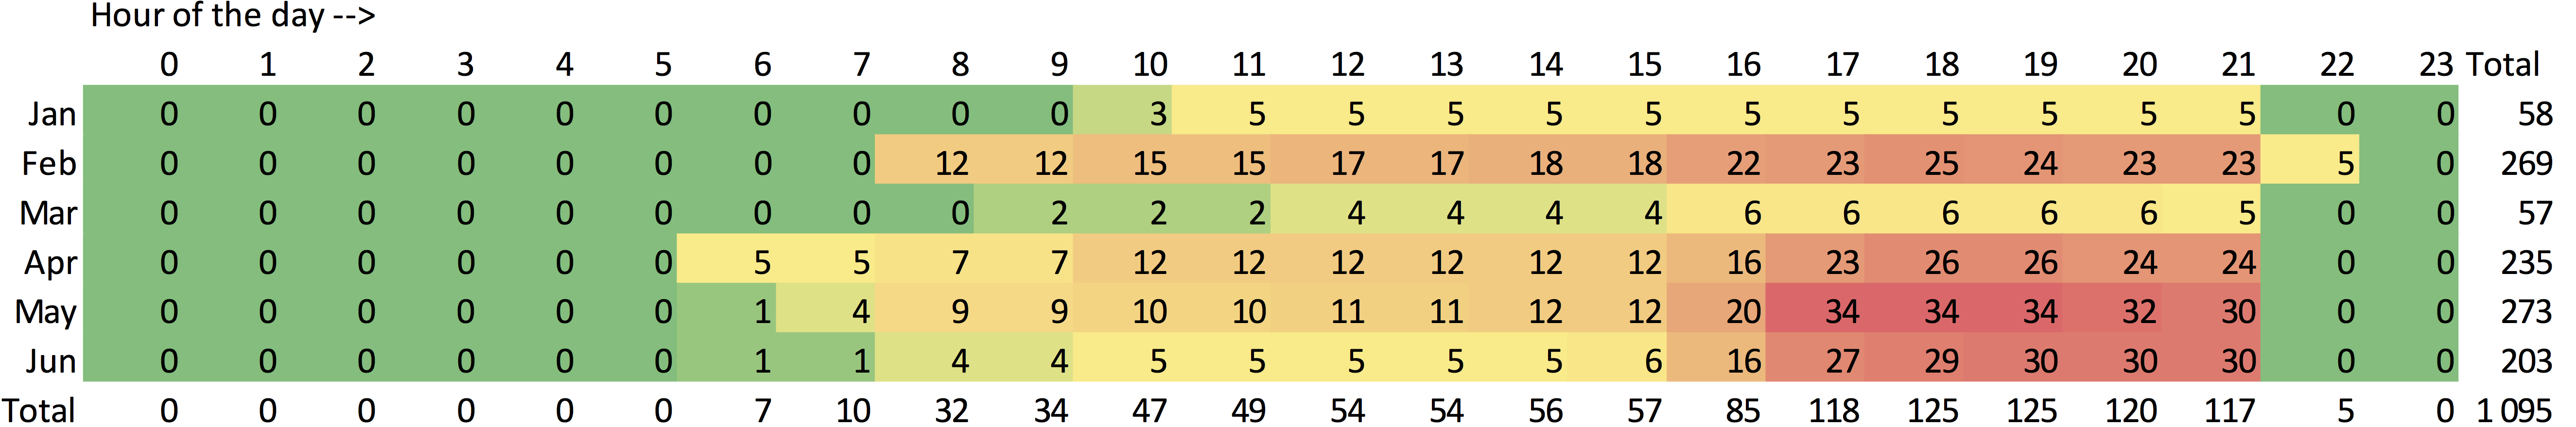
\includegraphics[width=1\linewidth]{FIG/Load_shedding_sum}
\caption[Total unserved energy due to load shedding for all hours per month Jan-Jun 2015 in GWh.]{Total unserved energy due to load shedding for all hours per month Jan-Jun 2015 in GWh \cite{CSIREnergyCentre2015}.}\label{Load_shedding_sum}
\end{figure}
It is a  hard requirement that plants meet the full electrical demand in the system. Figure~\ref{LoadScenarios} shows the daily average system load/demand in South Africa for the winter and summer period (2011). It can be seen that the summer profile has a particularly lower demand than the winter profile (up to \SI{15}{\percent} difference) and after a sharp rise at approx 7:00 the demand has a constant system load during the day due to commercial, agricultural and residential demand caused by air-conditioning, pool pumps and geysers, which comes to their peak demand at 20:00. In winter, there is an initial peak at 9:00 and a second at 19:00 mainly caused by residential customers due to electrical heating, lighting, cooking, geysers and pool pumps.

\begin{figure}[htbp]  
\centering
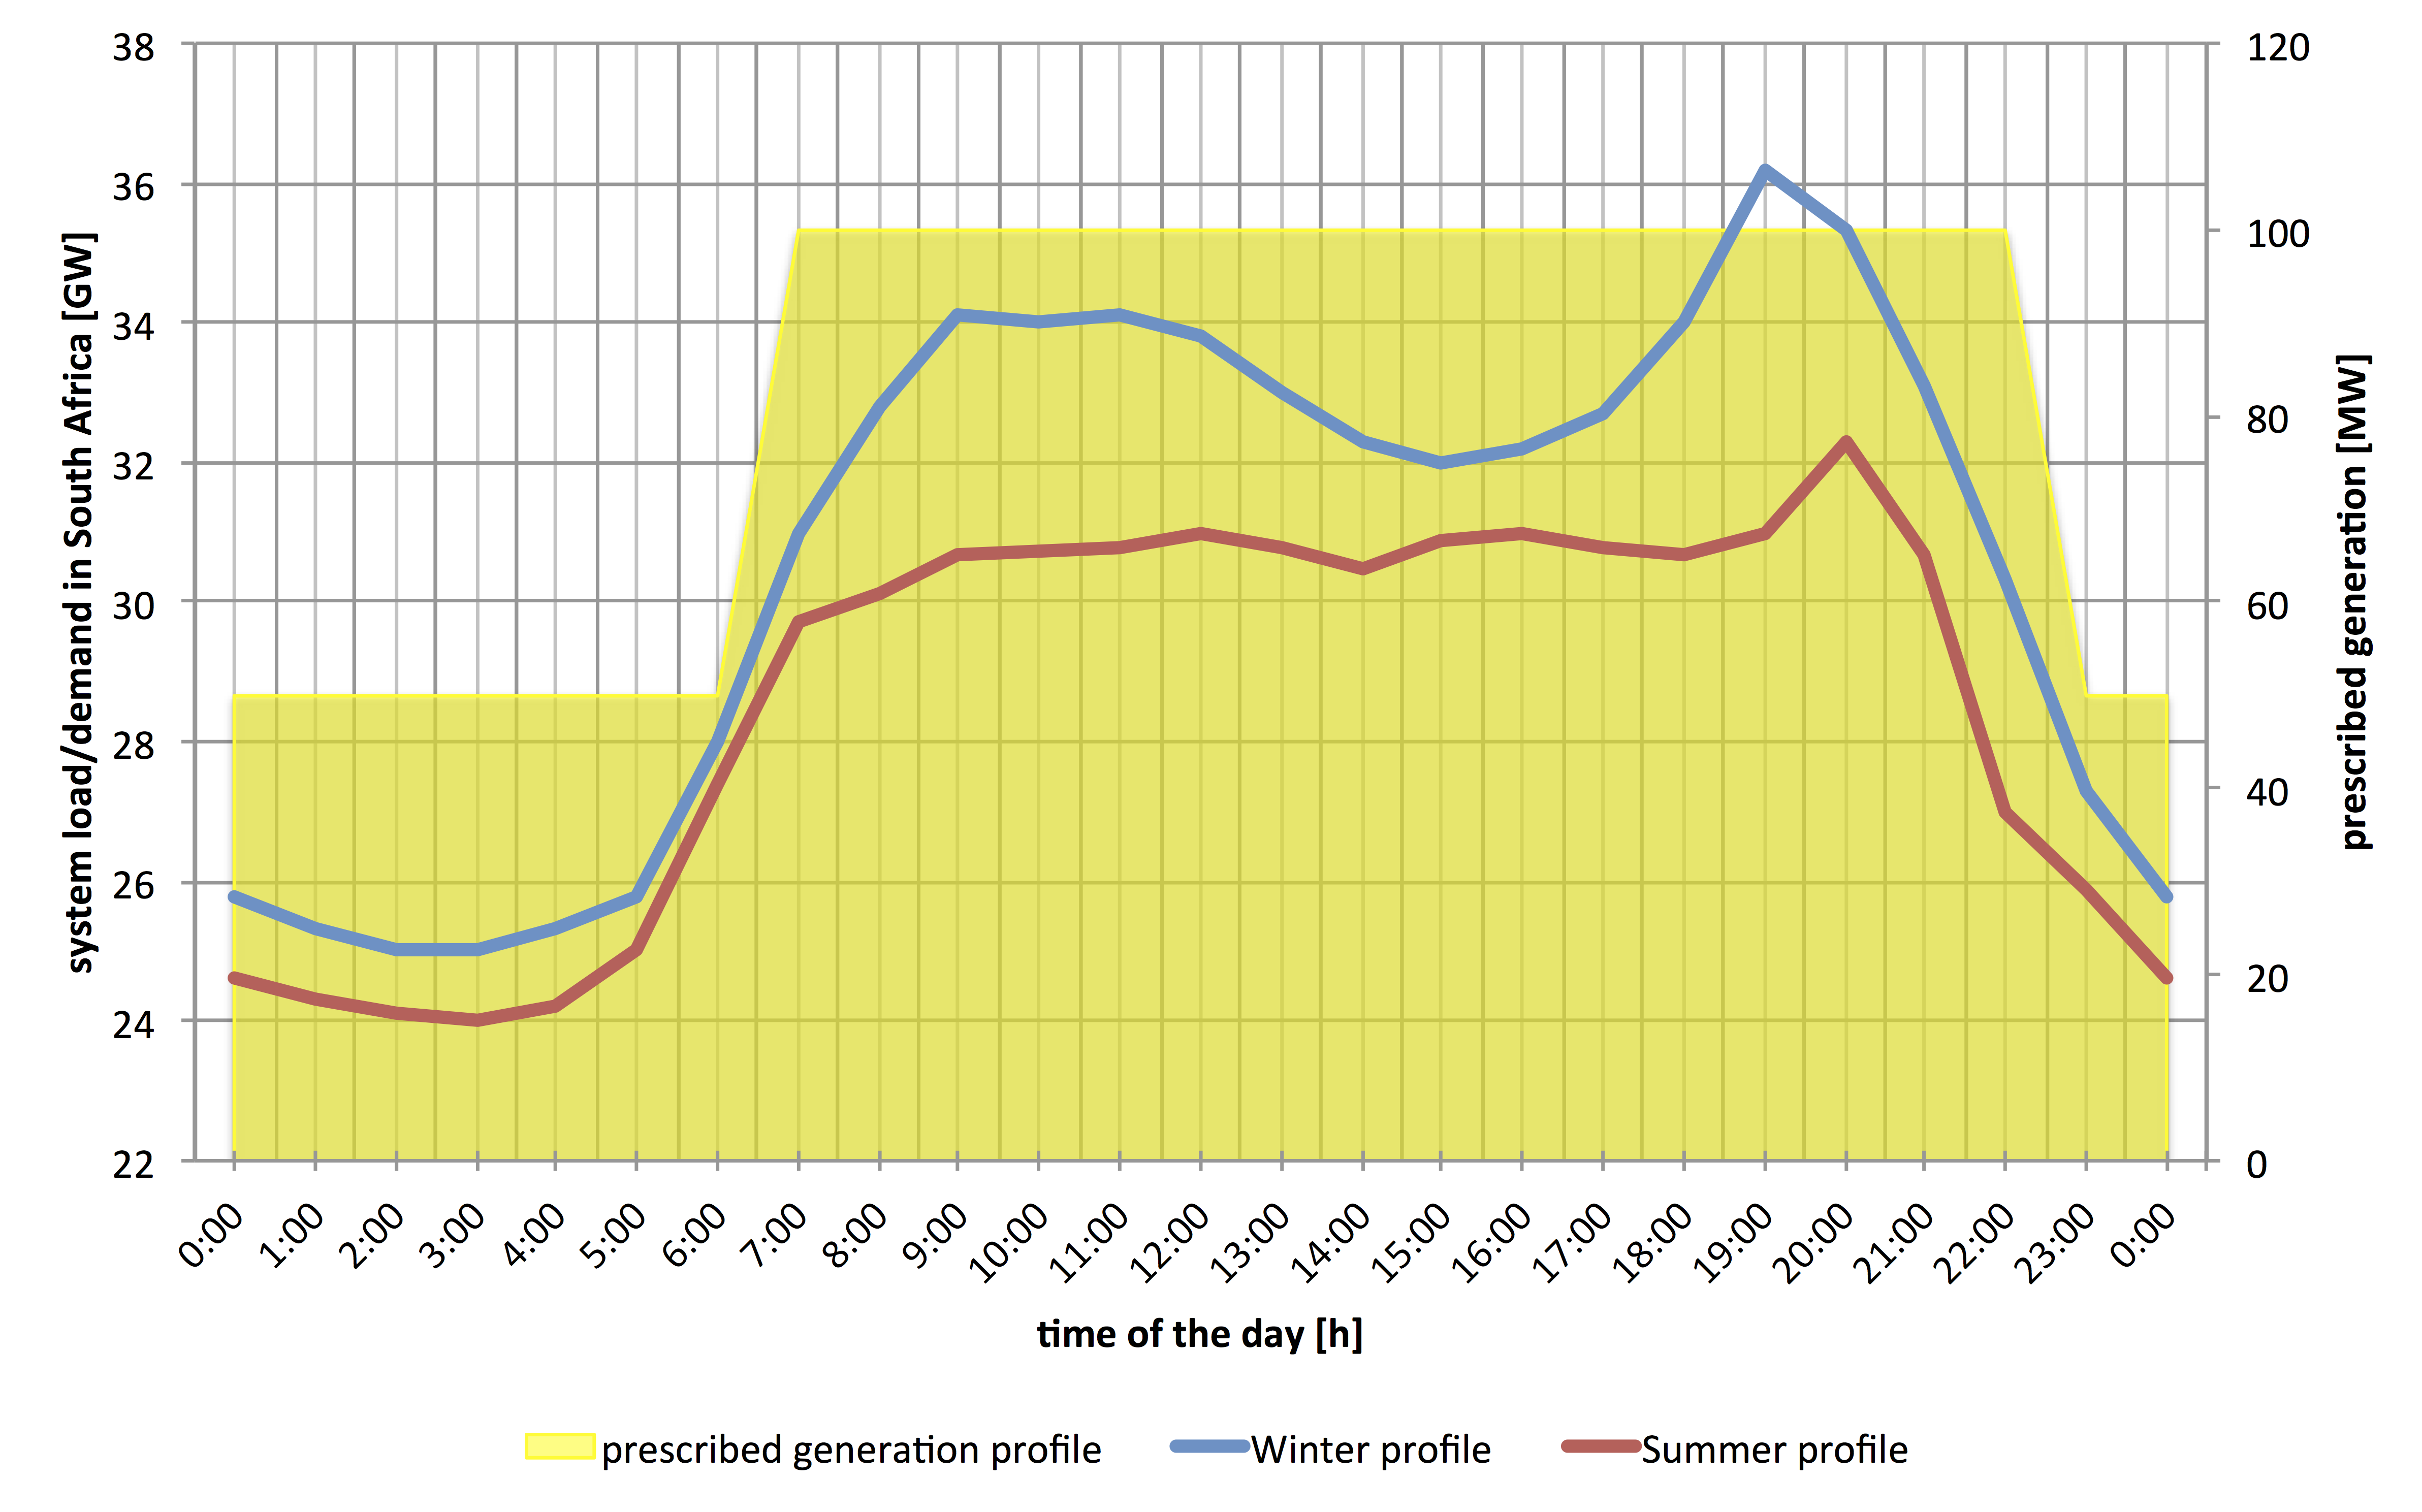
\includegraphics[width=1\linewidth]{FIG/LoadScenarios}
\caption[South Africa daily average system load/demand for summer and winter days, with prescribed generation profile.]{South Africa daily average system load/demand for summer and winter days, with prescribed generation profile.}\label{LoadScenarios}
\end{figure}

Considering the system load, the supply structure and the point of time by load shedding it is unequivocally that the South African power supply needs adjustable power plants which can support the demand during the evening hours till 22:00 in particular. 

In order to support the South African power supply were it is needed, the for the comparison selected solar power plants are forced to cover a prescribed generation profile. The solar power plants must operate at full power output of \SI{100}{\mega\watt} from 7:00 to 22:00. When the system demand drops during the night, the plants reduce there output from 22:00 to 7:00 to \SI{50}{\mega\watt}. At a covering of \SI{100}{\percent} of the prescribed generation the solar power plants would produce \SI{711.75}{\giga\watt\hour} per year.

With consideration to solar energy is depending on weather and seasonal conditions the individual system design must handle \SI{90}{\percent} of the prescribed generation profile and with regard to the PV system whose module efficiency deteriorates over there lifetime it is just defined for the first year of the plants. It signifies that the power plants are forced to produce more than \SI{640575}{\mega\watt\hour} in the first year.

Usually, in feed-in contracts, the deliverable maximum net power output of power plants is fixed. Any overproduction is not covered by such contracts and is not remunerated. In order to generate exploitable and comparable results and considering standard feed-in contracts, the hourly power production is cut to the planned values and thus overproduction is not considered in this analysis.

The results of the solar power plant simulations will therefore evaluated and compared by the following quantitative measures:
\begin{itemize}
\item \textbf{Generation curve covering} [\si{\percent}]: The generation curve covering (GCC) is an effectiveness measure describing how closely the plant follows the prescribed generation curve over the full year. It is defined as:

\begin{equation}
\mbox{GCC} = \sum\limits_{t=1}^{8760} \frac{\mbox{prescribed generation at }t\mbox{ in MW}}{\mbox{actual plant net output at }t\mbox{ in MW}} \label{GL_GCC}
\end{equation} 

\item \textbf{Levelized cost of electricity} [USD/\si{\mega\watt\hour}]: The levelized cost of electricity (LCOE) represents the total project life-cycle costs. It is the present value of project costs expressed in USD per megawatt-hour of electricity generated by the system over its life.
\end{itemize}
These performance and financial parameter are the only releavant indicator for the evaluation in this thesis, other indicators can be seen as supplement. 

It must be noted, that there is an important difference between the GCC and the widely-used \emph{capacity factor} (CF). The CF is the ratio of the system's electrical net output in the first year of operation to the nameplate output (CSP) or peak output (PV), which is equivalent to the quantity of energy the system would generate if it operated at its nameplate capacity for every hour of the year \cite{NREL2015a}. The GCC is calculated from the sum value of prescribed generation coverage in each hour of the year. 
\pagebreak 
